\begin{frame}
    \frametitle{SD... ¿qué?}
    
    
    \begin{columns}[c]
		\column{220pt}
		\begin{block}{¿Qué es la SDL?}
            \begin{itemize}
                \item Librería multimedia para aplicaciones 2D
                \item Escrita en lenguaje C
                \item Compatible con multitud de lenguajes (C, C++, Python...)
                \item Multiplataforma (Linux, Windows, Mac, PSP...)
                \item Completamente libre (LGPL)
            \end{itemize}            
        \end{block}
        
		\column{100pt}
		\begin{center}
			
\includegraphics[scale=0.2]{img/sdl.jpeg}
		\end{center}
	\end{columns}
    
    \begin{center}
        Mucha más información en http://osl.uca.es/wikijuegos
    \end{center}
\end{frame}

\begin{frame}
    \frametitle{Características}
    
    
    \begin{columns}[c]
		\column{160pt}
		\begin{block}{Lo que SÍ ofrece SDL}
            \begin{itemize}
                \item Vídeo
                \item Entrada
                \item Sonido
                \item Red
                \item Fuentes
                \item CD-ROM
                \item Control de tiempo
            \end{itemize}            
        \end{block}
        
		\column{160pt}
        
        \begin{alertblock}{Lo que NO ofrece SDL}
            \begin{itemize}
                \item Física
                \item Colisiones
                \item Inteligencia Artificial
                \item Gestión de recursos
                \item Animaciones
                \item GUI
                \item Aceleración por hardware
            \end{itemize}            
        \end{alertblock}
		
	\end{columns} 
\end{frame}


\begin{frame}
    \frametitle{Blitting}
    
    
    \begin{block}{Capas}
        \begin{itemize}
            \item Una SDL\_Surface es una capa sobre la que dibujar
            \item La SDL\_Surface principal representa la pantalla
            \item Cargamos imágenes en una SDL\_Surface
            \item Volcar una superficie sobre otra se llama \textbf{Blitting}
            \item Volcando superficies componemos la escena
        \end{itemize}            
    \end{block}

\end{frame}


\begin{frame}
    \frametitle{Blitting - Ejemplo}

    \begin{center}
		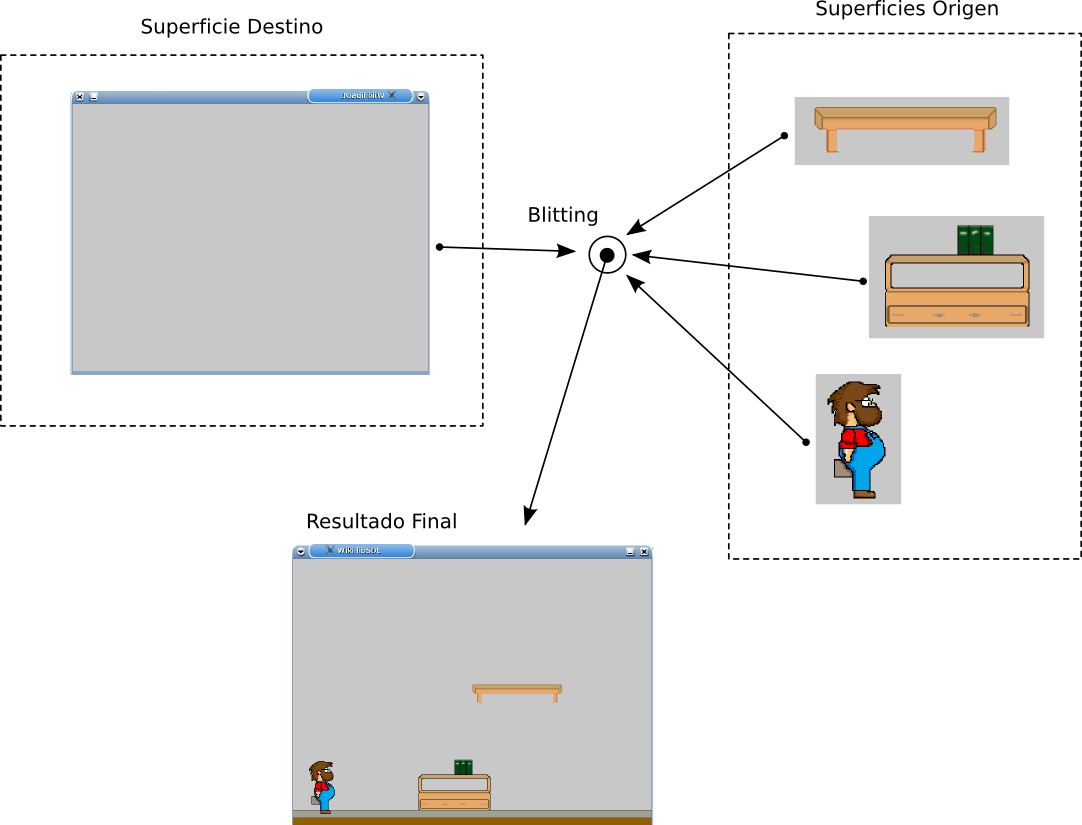
\includegraphics[scale=0.5]{img/Blitting.png}
	\end{center}
    
\end{frame}

\begin{frame}
    \frametitle{El Flipping y el doble buffer}
    
	\begin{block}{Doble buffer}
        \begin{itemize}
            \item Tenemos dos superficies: pantalla y auxiliar
            \item Hacemos blitting sobre la auxiliar
            \item Terminamos de componer la escena
            \item Intercambiamos pantalla y auxiliar
            \item Evitamos un horroroso parpadeo
        \end{itemize}            
    \end{block}
    
\end{frame}

\begin{frame}
    \frametitle{Flipping - Ejemplo}

    \begin{center}
		
\includegraphics[scale=2]{img/flipping.png}
	\end{center}
    
\end{frame}
